\setchapterpreamble[u]{\margintoc}
\chapter{Match to Hydrodynamics}
\labch{matching}

\begin{preview}[]
Impact parameter and energy dependence are implemented in the {\sffamily MV} model. The Landau matching is explained and resulting local rest frame energy density and flow velocity are studied. The centrality selection procedure is then presented.
\end{preview}

\section{Improved {\sffamily MV} model}
\subsubsection*{Impact parameter dependence}
Until now only central collisions were taken into consideration. In order to simulate non-central collisions, one simply employs the color charge density of the {\sffamily MV} model as\sidenote{With the notation
\begin{align*}
    r_\perp\overset{\Delta}{=}\sqrt{\left(x\pm\frac{b}{2}\right)^2+\left(y\pm\frac{b}{2}\right)^2},
\end{align*}
where $\vec{x}_\perp=(x,y)$. 
}
\begin{align*}
    \rho^a(\vec{x}_\perp)\mapsto \sigma(r_\perp)\rho^a(\vec{x}_\perp),
\end{align*}
modulated by a Woods-Saxon distribution given by\sidenote{For a {\sffamily Au} nucleus, the radius is $r_0=6.38$ fm and the surface thickness $a=0.535$ fm \cite{romatschke}.
}
\begin{align*}
    \sigma(r_\perp)\overset{\Delta}{=}\dfrac{1}{1+\exp{\dfrac{r_\perp-r_0}{a}}}.
\end{align*}

\vspace{-0.3cm}

\begin{figure}[!hbt]
	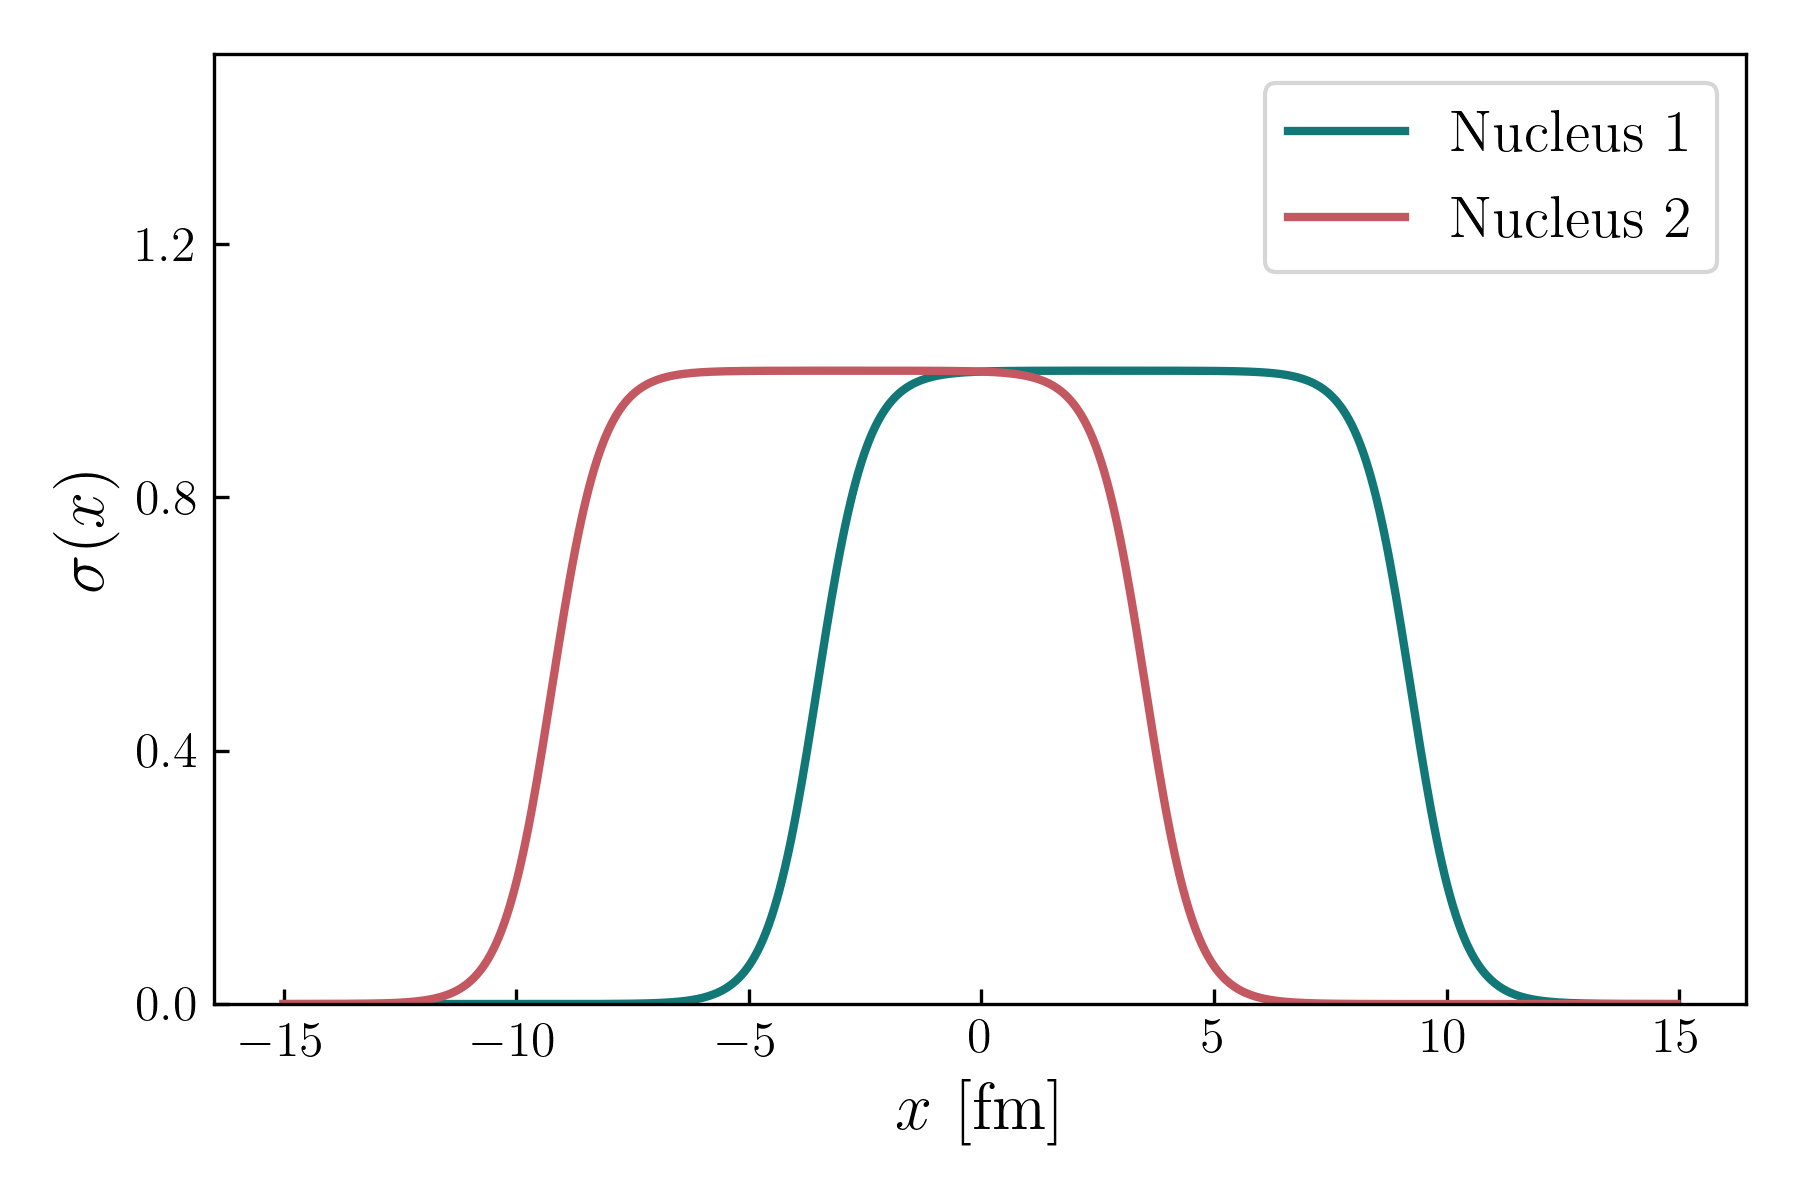
\includegraphics[width=\textwidth]{woods_saxon_auau_200.png}
	\caption{\normalsize Woods-Saxon distribution $\sigma(x,y)$ as a function of $x$ at $y=0$ for a $10$-$20\%$ centrality event having $b=5.7$ fm.} 
\end{figure}

Off-central collisions are thus obtained by shifting the transverse radius\sidenote{For example, with $b/2$ for nucleus $\textsf{1}$ and $-b/2$ for nucleus $\textsf{2}$.}with $\pm b/2$.

\begin{figure}[!hbt]
	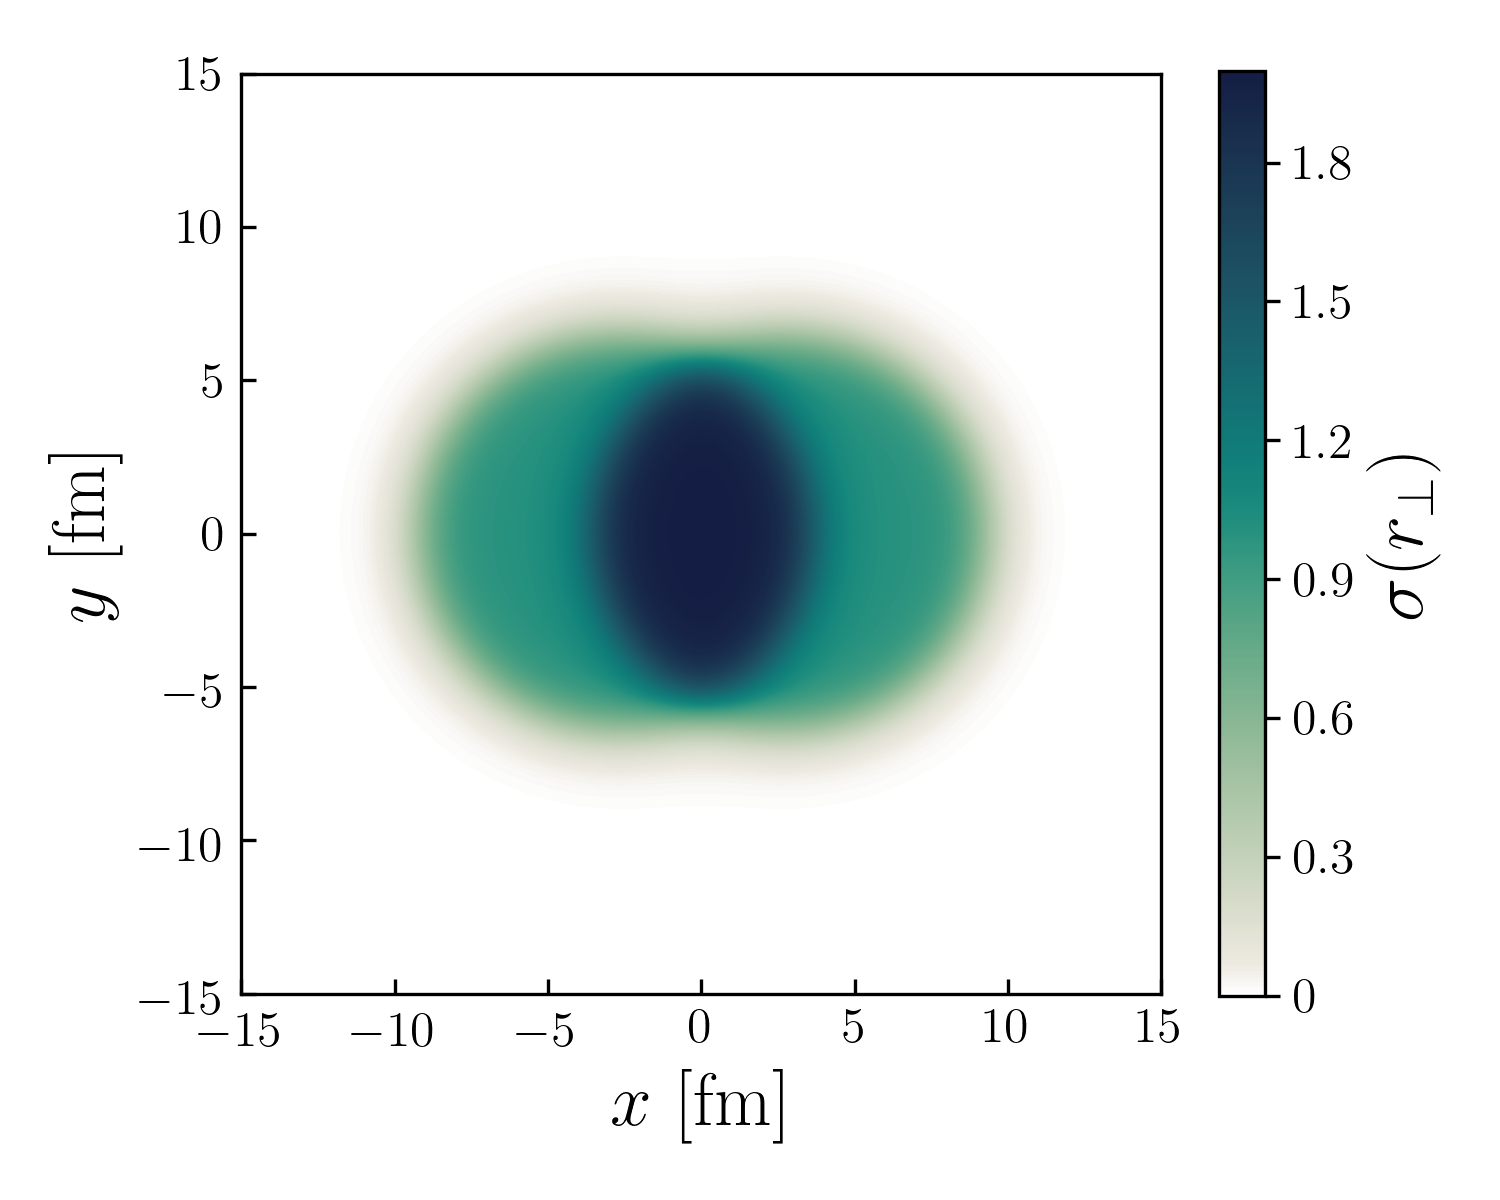
\includegraphics[width=0.833\textwidth]{woods_saxon_3d_auau_200.png}
	\caption{\normalsize Woods-Saxon distribution $\sigma(r_\perp)$ in the transverse plane $(x,y)$ for an event within $10$-$20\%$ centrality having $b=5.7$ fm.} 
\end{figure}
 
\subsubsection*{Energy dependence}
Instead of providing approximate values for the phenomenological parameters, one may use results borrowed from {\sffamily DIS} and express all the relevant parameters in terms $\sqrt{s_{\textsf{NN}}}$ and $A$ for a given system. More concisely, we are going to make use of {\sffamily\color{ming}geometrical scaling} which relates the saturation momentum of the proton $\textsf{Q}_{s,p}$ to the $x$ value of a parton belonging to the proton as\sidenote{This parametrization is used in the {\sffamily GWB} model of saturation \cite{gbw}. There exist more sophisticated models which incorporate the physics of saturation, see \cite{albacete} for a schematic overview.}
\begin{align*}
    \textsf{Q}_{s,p}^2=\textsf{Q}_0^2\left(\dfrac{x_0}{x}\right)^\lambda,
\end{align*}
with $x_0=3.04\cdot 10^{-4}$, $\lambda=0.288$ and $\textsf{Q}_0=1$ GeV, as extracted from fits to {\sffamily HERA} data\sidenote{Fits including charm quarks lead to different values for these parameters, resulting in a larger saturation scale \cite{lappidis}.}\cite{gbw}. If the momentum fraction $x$ is chosen to take an effective value as
\begin{align*}
    x=x_\text{eff}\approx \frac{\textsf{Q}_{s,p}}{\sqrt{s_{\textsf{NN}}}},
\end{align*}
one may deduce a parametrization of the saturation momentum in terms of energy as
\begin{align*}
    \textsf{Q}_{s, p}^{2}(\sqrt{s_{\textsf{NN}}}) \approx 0.13 \sqrt{s_{\textsf{NN}}} ^{0.25} \text{ GeV}^{2}.
\end{align*}
The saturation scale of a nucleus $\textsf{Q}_{s,A}$ with a given $A$ may be obtained from the saturation scale of the proton $\textsf{Q}_{s,p}$ through scaling with a geometric factor $\textsf{g}_A$ which is chosen to take the simple form\sidenote{See \cite{lappidis} for other possible extrapolations of the {\sffamily DIS} data on protons to nuclei.}
\begin{align*}
    \textsf{Q}_{s,A}^2=\textsf{g}_A\textsf{Q}_{s,p}^2\approx A^{1/3}\textsf{Q}_{s,p}^2.
\end{align*}
This eventually leads to the following parametrization of the saturation scale\sidenote{For a {\sffamily Au} nucleus with $A=197$ at {\sffamily RHIC} energies of $\sqrt{s_{\textsf{NN}}}=200$ GeV, the saturation scale yields $\textsf{Q}_{s,A}\approx 1.68$ GeV.}
\begin{align*}
    \textsf{Q}_{s,A}^2\approx 0.13 A^{1/3} \sqrt{s_{\textsf{NN}}} ^{0.25} \text{ GeV}^{2}.
\end{align*}
Once the saturation scale is fixed, the coupling constant may be computed from
\begin{align*}
    g^2=\dfrac{\alpha_s(\textsf{Q}_{s,A})}{4\pi},
\end{align*}
where the running coupling constant is given by\sidenote{With the number of flavours $N_f=3$ and the {\sffamily QCD} scale $\Lambda_\textsf{QCD}\approx 200$ GeV for $\textsf{SU}(3)$. For $\textsf{Q}_{s,A}\approx 1.68$ GeV, this yields a coupling constant of $g\approx 2.15$.}
\begin{align*}
    \alpha_{s}(\textsf{Q}_{s,A}^{2})=\dfrac{1}{\dfrac{33-3N_f}{12\pi} \ln{\dfrac{\textsf{Q}_{s,A}^{2}}{\Lambda_{\textsf{QCD}}^{2}}}}.
\end{align*}
The relation between the saturation scale $\textsf{Q}_{s,A}$ and {\sffamily MV} model parameter $\mu$ is influenced in a non-trivial manner by the number of color sheets $N_s$ and {\sffamily IR} regulator $m$. In \cite{lappidis}, it yields\sidenote{This results in $\mu\approx 0.45$ GeV {\sffamily MV} parameter for a regulator $m\approx 0.21$ GeV.}$\textsf{Q}_{s,A}\approx 0.8g^2\mu$ for $N_s=50$ and $m=0.1g^2\mu$.

\section{Landau matching}
The Glasma exhibits pressure anisotropy and within a classical description,\sidenote{Using non-Abelian Yang-Mills theory.}it may never reach isotropy. Nevertheless, the produced {\sffamily QGP} may very well be described by employing an ideal hydrodynamics evolution \cite{kolb, huovinen}, during which the medium is assumed to be isotropic. In order to match this distinct and irreconcilable scenarios, we are going to discard information from the Glasma energy-momentum tensor.\sidenote{By neglecting the components which would deviate the system from equilibrium.}One may construct an ideal energy-momentum tensor through a procedure named {\sffamily\color{ming} Landau matching} as\sidenote{Here $\textsf{P}$ represents the pressure and may be computed once an equation of state is provided, namely $\textsf{P}=\textsf{P}(\varepsilon,T)$.}
\begin{align*}
    \textsf{T}^{\mu \nu}=(\varepsilon_\textsf{LRL}+\textsf{P}) u^{\mu} u^{\nu}-\textsf{P} g^{\mu \nu}=\textsf{Diag}\{\varepsilon_\textsf{LRL}, \textsf{P}, \textsf{P}, \textsf{P}\},
\end{align*}
where the local rest frame ({\sffamily LRF}) energy density $\varepsilon_\textsf{LRL}$ and the flow velocity $u^\mu$ may be obtained by solving the eigenvalue equation\sidenote{Where $T^{\mu\nu}$ is the energy-momentum tensor of the Glasma fields. One must only choose time-like flow vectors
\begin{align*}
    u^\mu u_\mu=1.
\end{align*}
}
\begin{align}\label{matt}
    T_{\nu}^{\mu} u^{\nu}=\varepsilon_\textsf{LRL} u^{\mu}.
\end{align}

\begin{note}
For a dissipative fluid which is near equilibrium, one may decompose the energy-momentum tensor as\sidenote{Once dissipation exhibits itself, thermodynamic quantities, which were well defined only for a fluid at local thermal equilibrium, may no longer be used.}
\begin{align*}
    T^{\mu\nu}=T^{\mu\nu}_\text{ideal}+\delta T^{\mu\nu}.
\end{align*}
Nevertheless, one may artificially assure local equilibrium by imposing the Landau matching condition\sidenote{Valid for an arbitrary $u^\mu$.}through
\begin{align*}
    u_\mu u_\nu \delta T^{\mu\nu}=0,
\end{align*}
which further yields\sidenote{In this way, the equilibrium component of $T^{\mu\nu}$ may be constructed from the local rest frame energy $\varepsilon_\textsf{LRL}$.}
\begin{align*}
    \varepsilon_\textsf{LRL}=u_\mu u_\nu T^{\mu\nu}.
\end{align*}
For a dissipative system in which both energy and particle diffusion coexist, one may define the {\sffamily LRL}\sidenote{For the ideal fluid, a {\sffamily LRF} was simply the frame in which the fluid volume element was at rest and both the energy and particle flows were null.}in multiple ways. Nevertheless, there exist two simple choices: the Eckart frame, where the energy flow is null, and the Landau frame, in which particle flow vanishes.\sidenote{This choice is more appropriate for ultrarelativistic heavy-ion collisions since they take place at negligible net baryon current.}In the Landau frame, the flow velocity $u^\mu$ is chosen to be along the energy flow velocity $T^{\mu\nu}u_\nu$, that is
\begin{align*}
    u_\nu T^{\mu\nu}=\varepsilon_\textsf{LRL}u^\mu.
\end{align*}
\end{note}

\begin{figure*}[h!]
	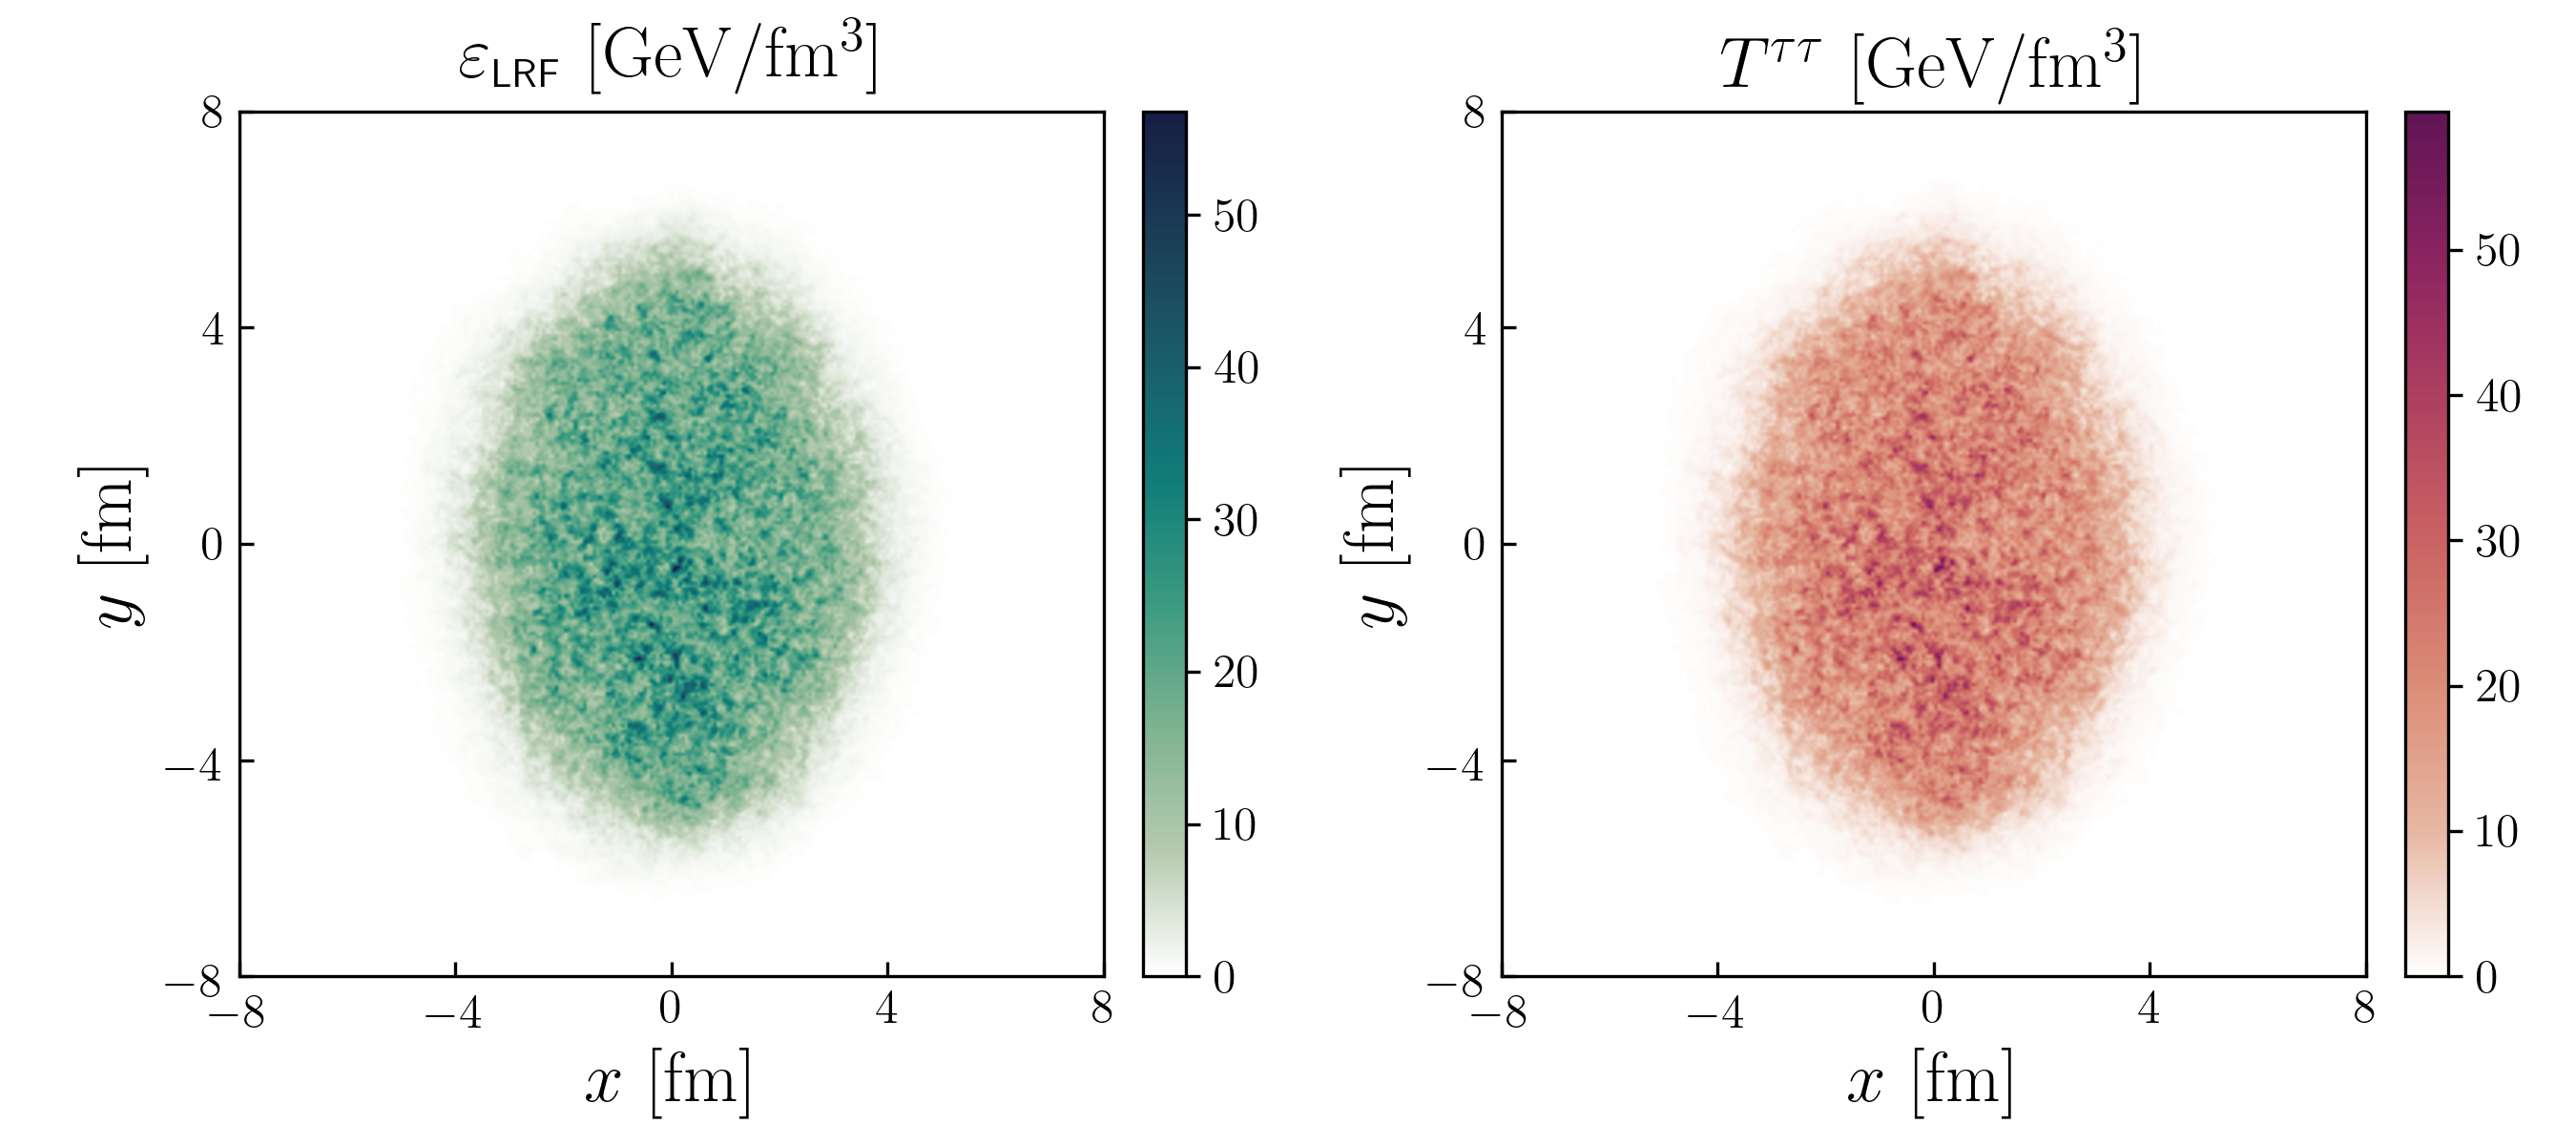
\includegraphics{images/ed_lrl_lab_auau_200_dpi_300.png}
	\caption{\normalsize Qualitative comparison between the local rest frame $\varepsilon_\textsf{LRL}$ and $T^{\tau\tau}$ component of the Glasma energy-momentum tensor, evaluated at $\tau_\mathrm{switch}=0.4$ fm/c for a $10$-$20\%$ centrality event with $b=5.7$ fm.}
\end{figure*}

In the boost-invariant approximation, one may further neglect the longitudinal flow component\sidenote{As emphasized in \cite{mcdonald} and showed in \cite{mcdolandflow}, this component turns out to also be of relevance.}$u^\eta=0$. Hence, the problem reduces to finding the eigenvalues $\varepsilon_\textsf{LRL}$ and eigenvectors $(u^\tau, u^x, u^y)$ of a $3\times 3$ sub-matrix of $T^{\mu\nu}$. 

One may define flow velocities weighted with respect to the energy density as\sidenote{Where $w^\perp\overset{\Delta}{=}(w^x,w^y)$ and similarly for $u^\perp$.}
\begin{align*}
    w^\perp\overset{\Delta}{=}\dfrac{\varepsilon_\textsf{LRL}}{\langle\varepsilon_\textsf{LRL}\rangle}u^\perp.
\end{align*}

\vspace{-0.5cm}

\begin{figure*}[h!]
	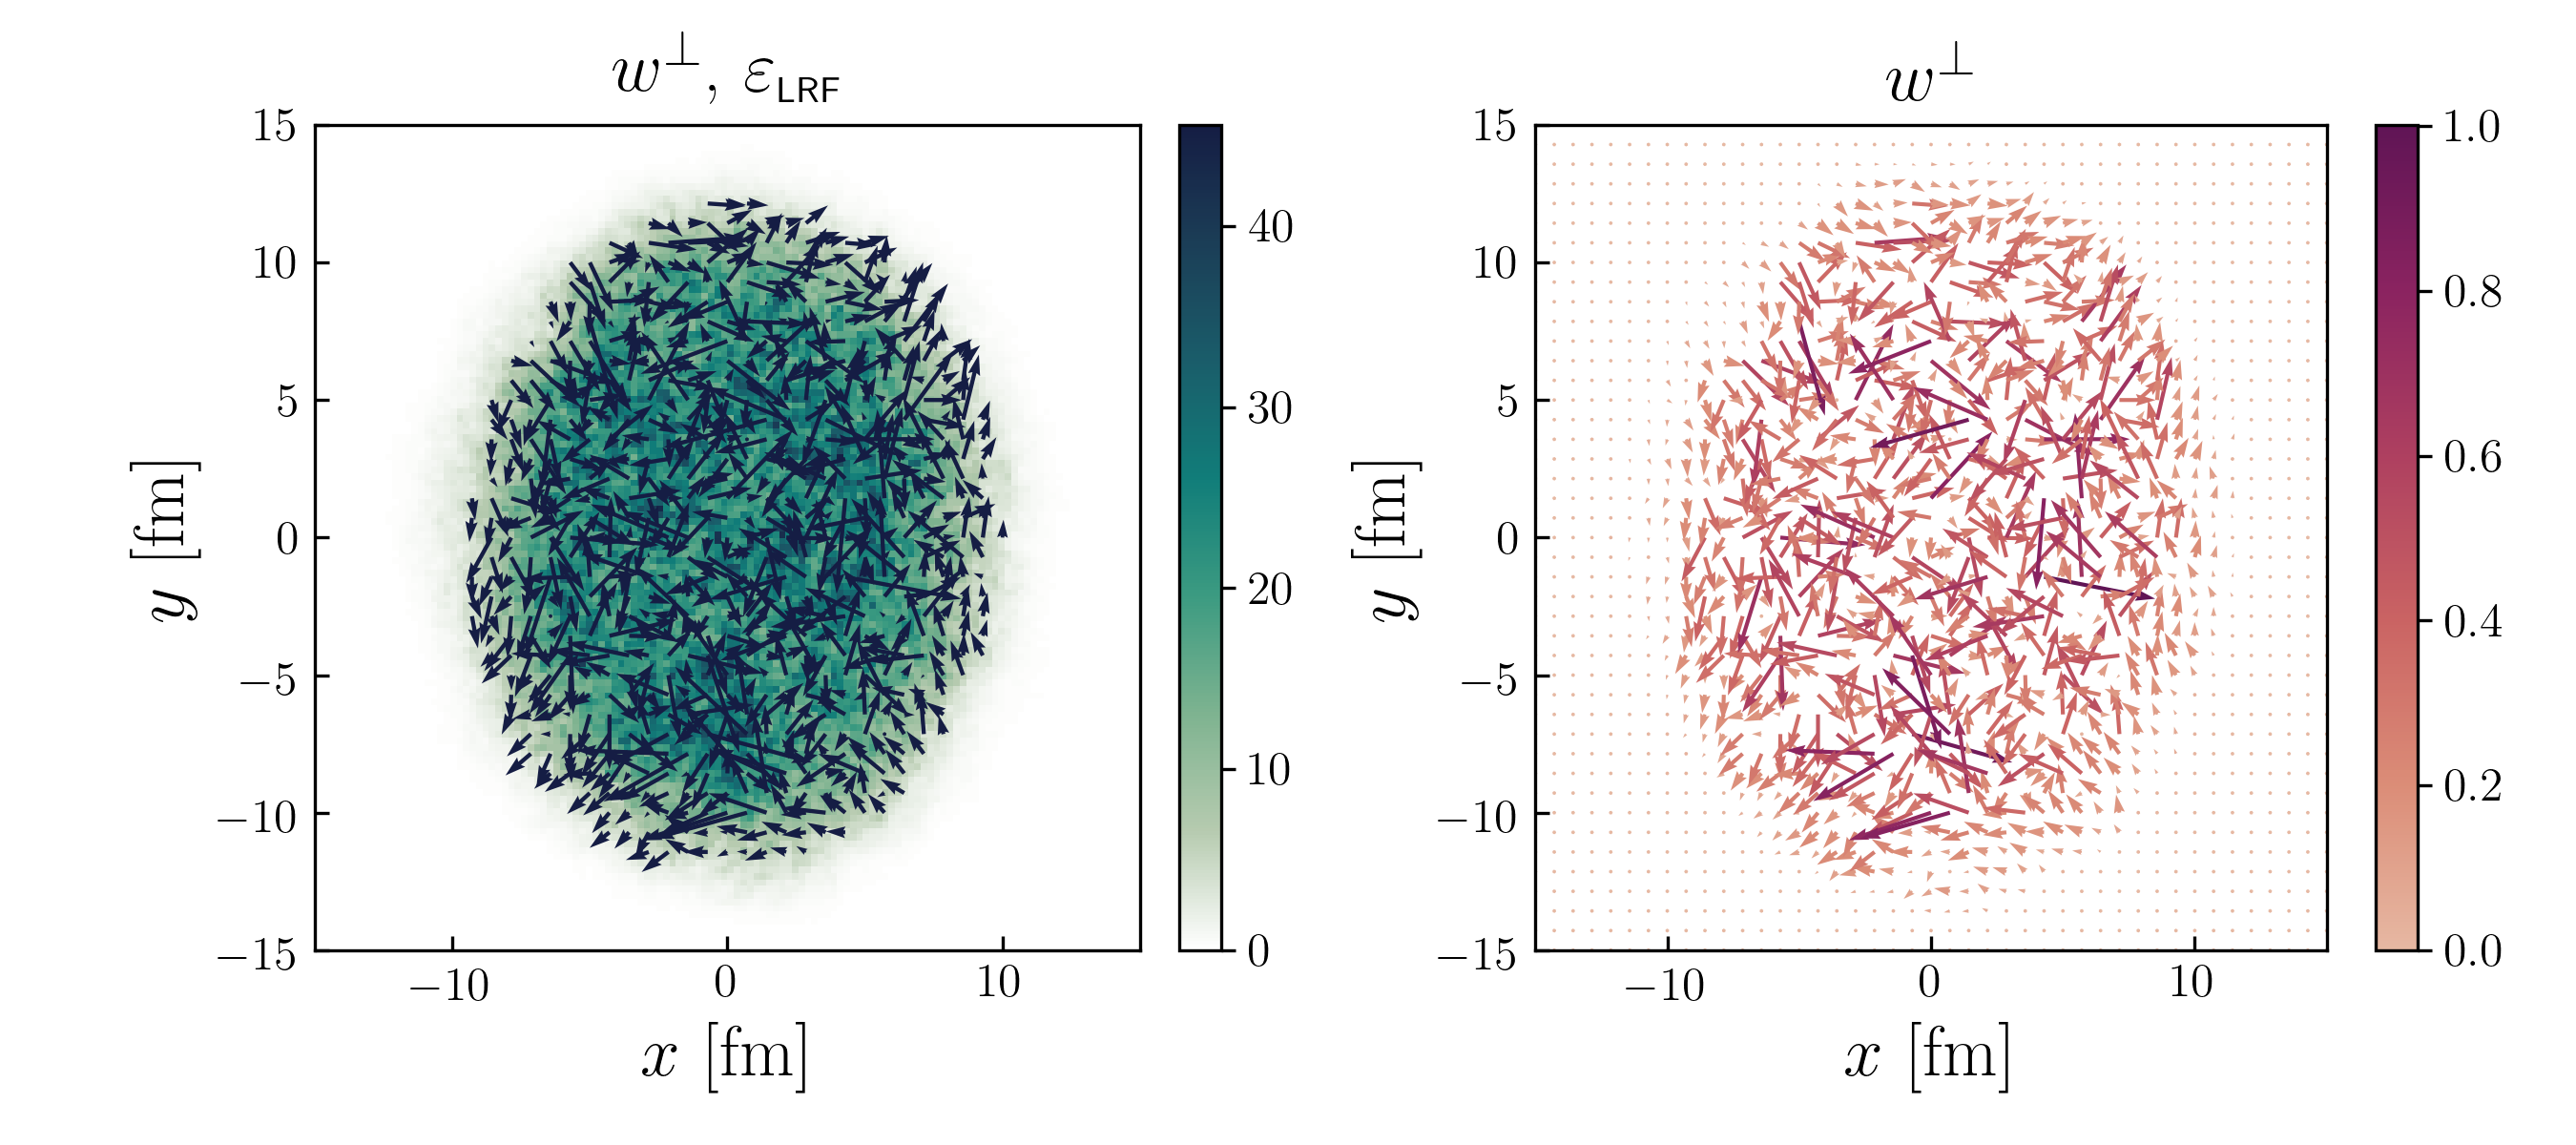
\includegraphics{images/ed_u_auau_200_dpi_300.png}
	\caption{\normalsize Weighted flow velocity $w^\perp$ superimposed over the local rest frame $\varepsilon_\textsf{LRL}$, evaluated at $\tau_\mathrm{switch}=0.4$ fm/c for a $5$-$10\%$ centrality event with $b=3.7$ fm.}
\end{figure*}

\begin{figure}[!hbt]
	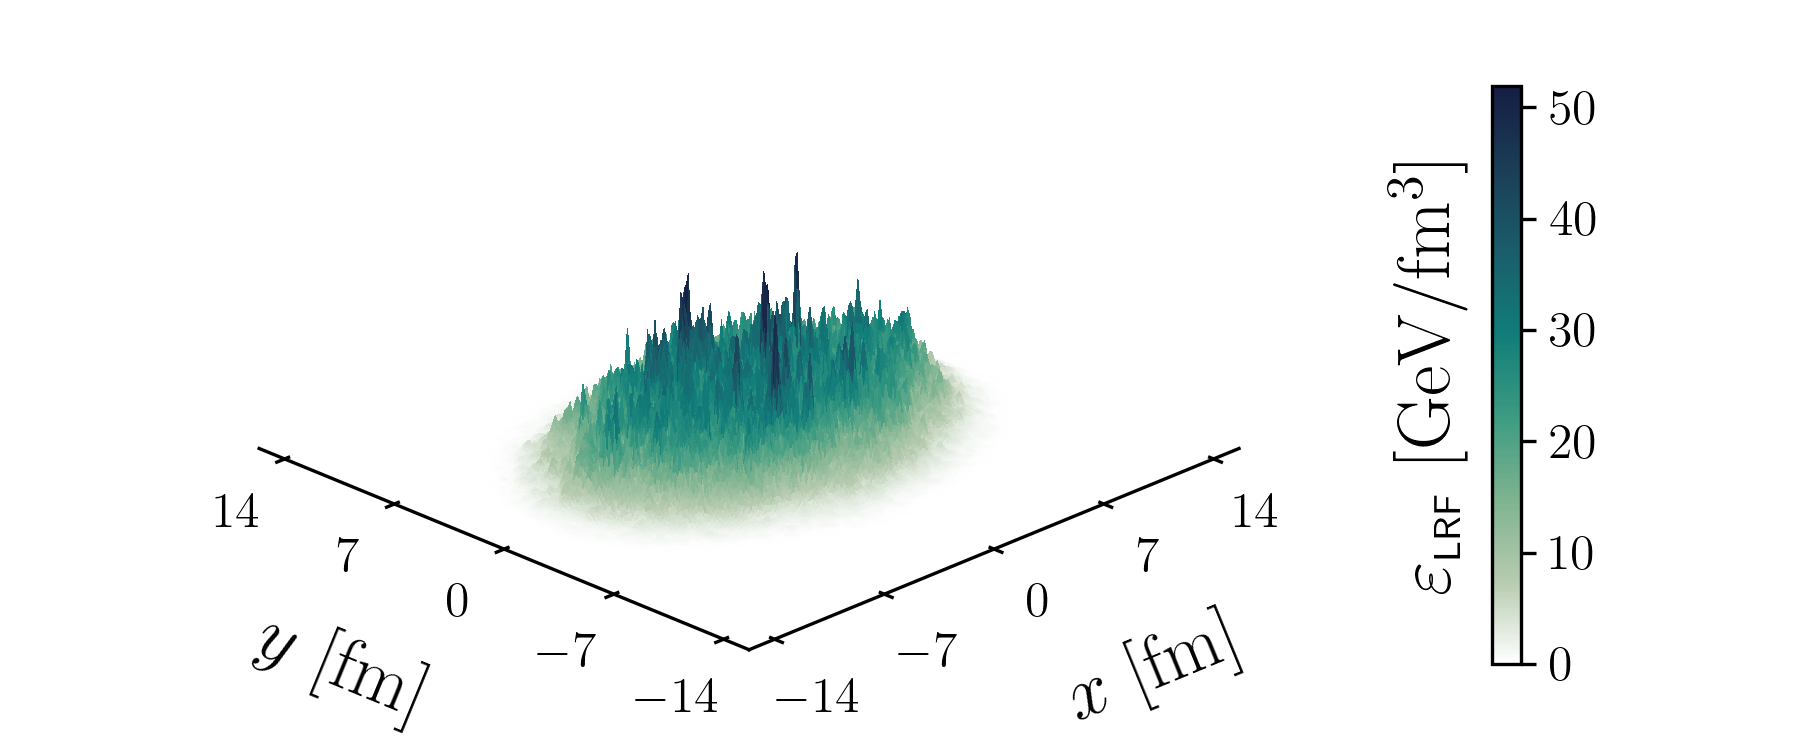
\includegraphics[trim=40 0 40 0,clip,width=\textwidth]{ed_3d.png}
	\caption{\normalsize Energy density in the local rest frame $\varepsilon_\textsf{LRL}$ as a function of the transverse coordinates, evaluated at $\tau_\mathrm{switch}=0.4$ fm/c for a $10$-$20\%$ centrality event with $b=5.7$ fm. One may notice spikes arising from the highly dense regions of the Glasma.} 
\end{figure}

\section{Centrality selection}
Each event requires an impact parameter as input. In order to mimic the minimum bias centrality selection, one needs to simulate many events\sidenote{We simulated $5\cdot 10^{4}$ events.}with impact parameters\sidenote{In the range $b\in(0,3r_0)$, that is $b\approx 0\divisionsymbol 18$ fm.}randomly distributed according to
\begin{align*}
    \textsf{P}(b)db=\dfrac{bdb}{b^2_\text{max}/2}.
\end{align*}
The centrality selection should be performed in terms of the final charged particles multiplicity $dN_\text{ch}/d\eta$ but we are going to apply the centrality cuts before the hydrodynamic evolution\sidenote{We are going to make use of the fact that there exists a good correlation between the initial energy in the central pseudorapidity region and the final charged multiplicity.}since performing hydrodynamics simulations on such a large number of events is computationally expensive and time consuming. \\
The Glasma fields are evolved until $\tau_\text{swith}=0.4$ fm/c. We already observed that for proper times $\tau>0.1$ fm/c the expansion of the system is of Bjorken type. Hence, the energy density at mid-pseudorapidity of the Glasma may be expressed as \cite{bjorken}
\begin{align*}
    \varepsilon(\tau)\approx \frac{1}{\textsf{S}_\perp}\left(\frac{1}{\tau}\frac{dE_\perp}{d\eta}\right).
\end{align*}

\vspace{-0.5cm}

\begin{figure*}[h!]\labfig{centralitycut}
	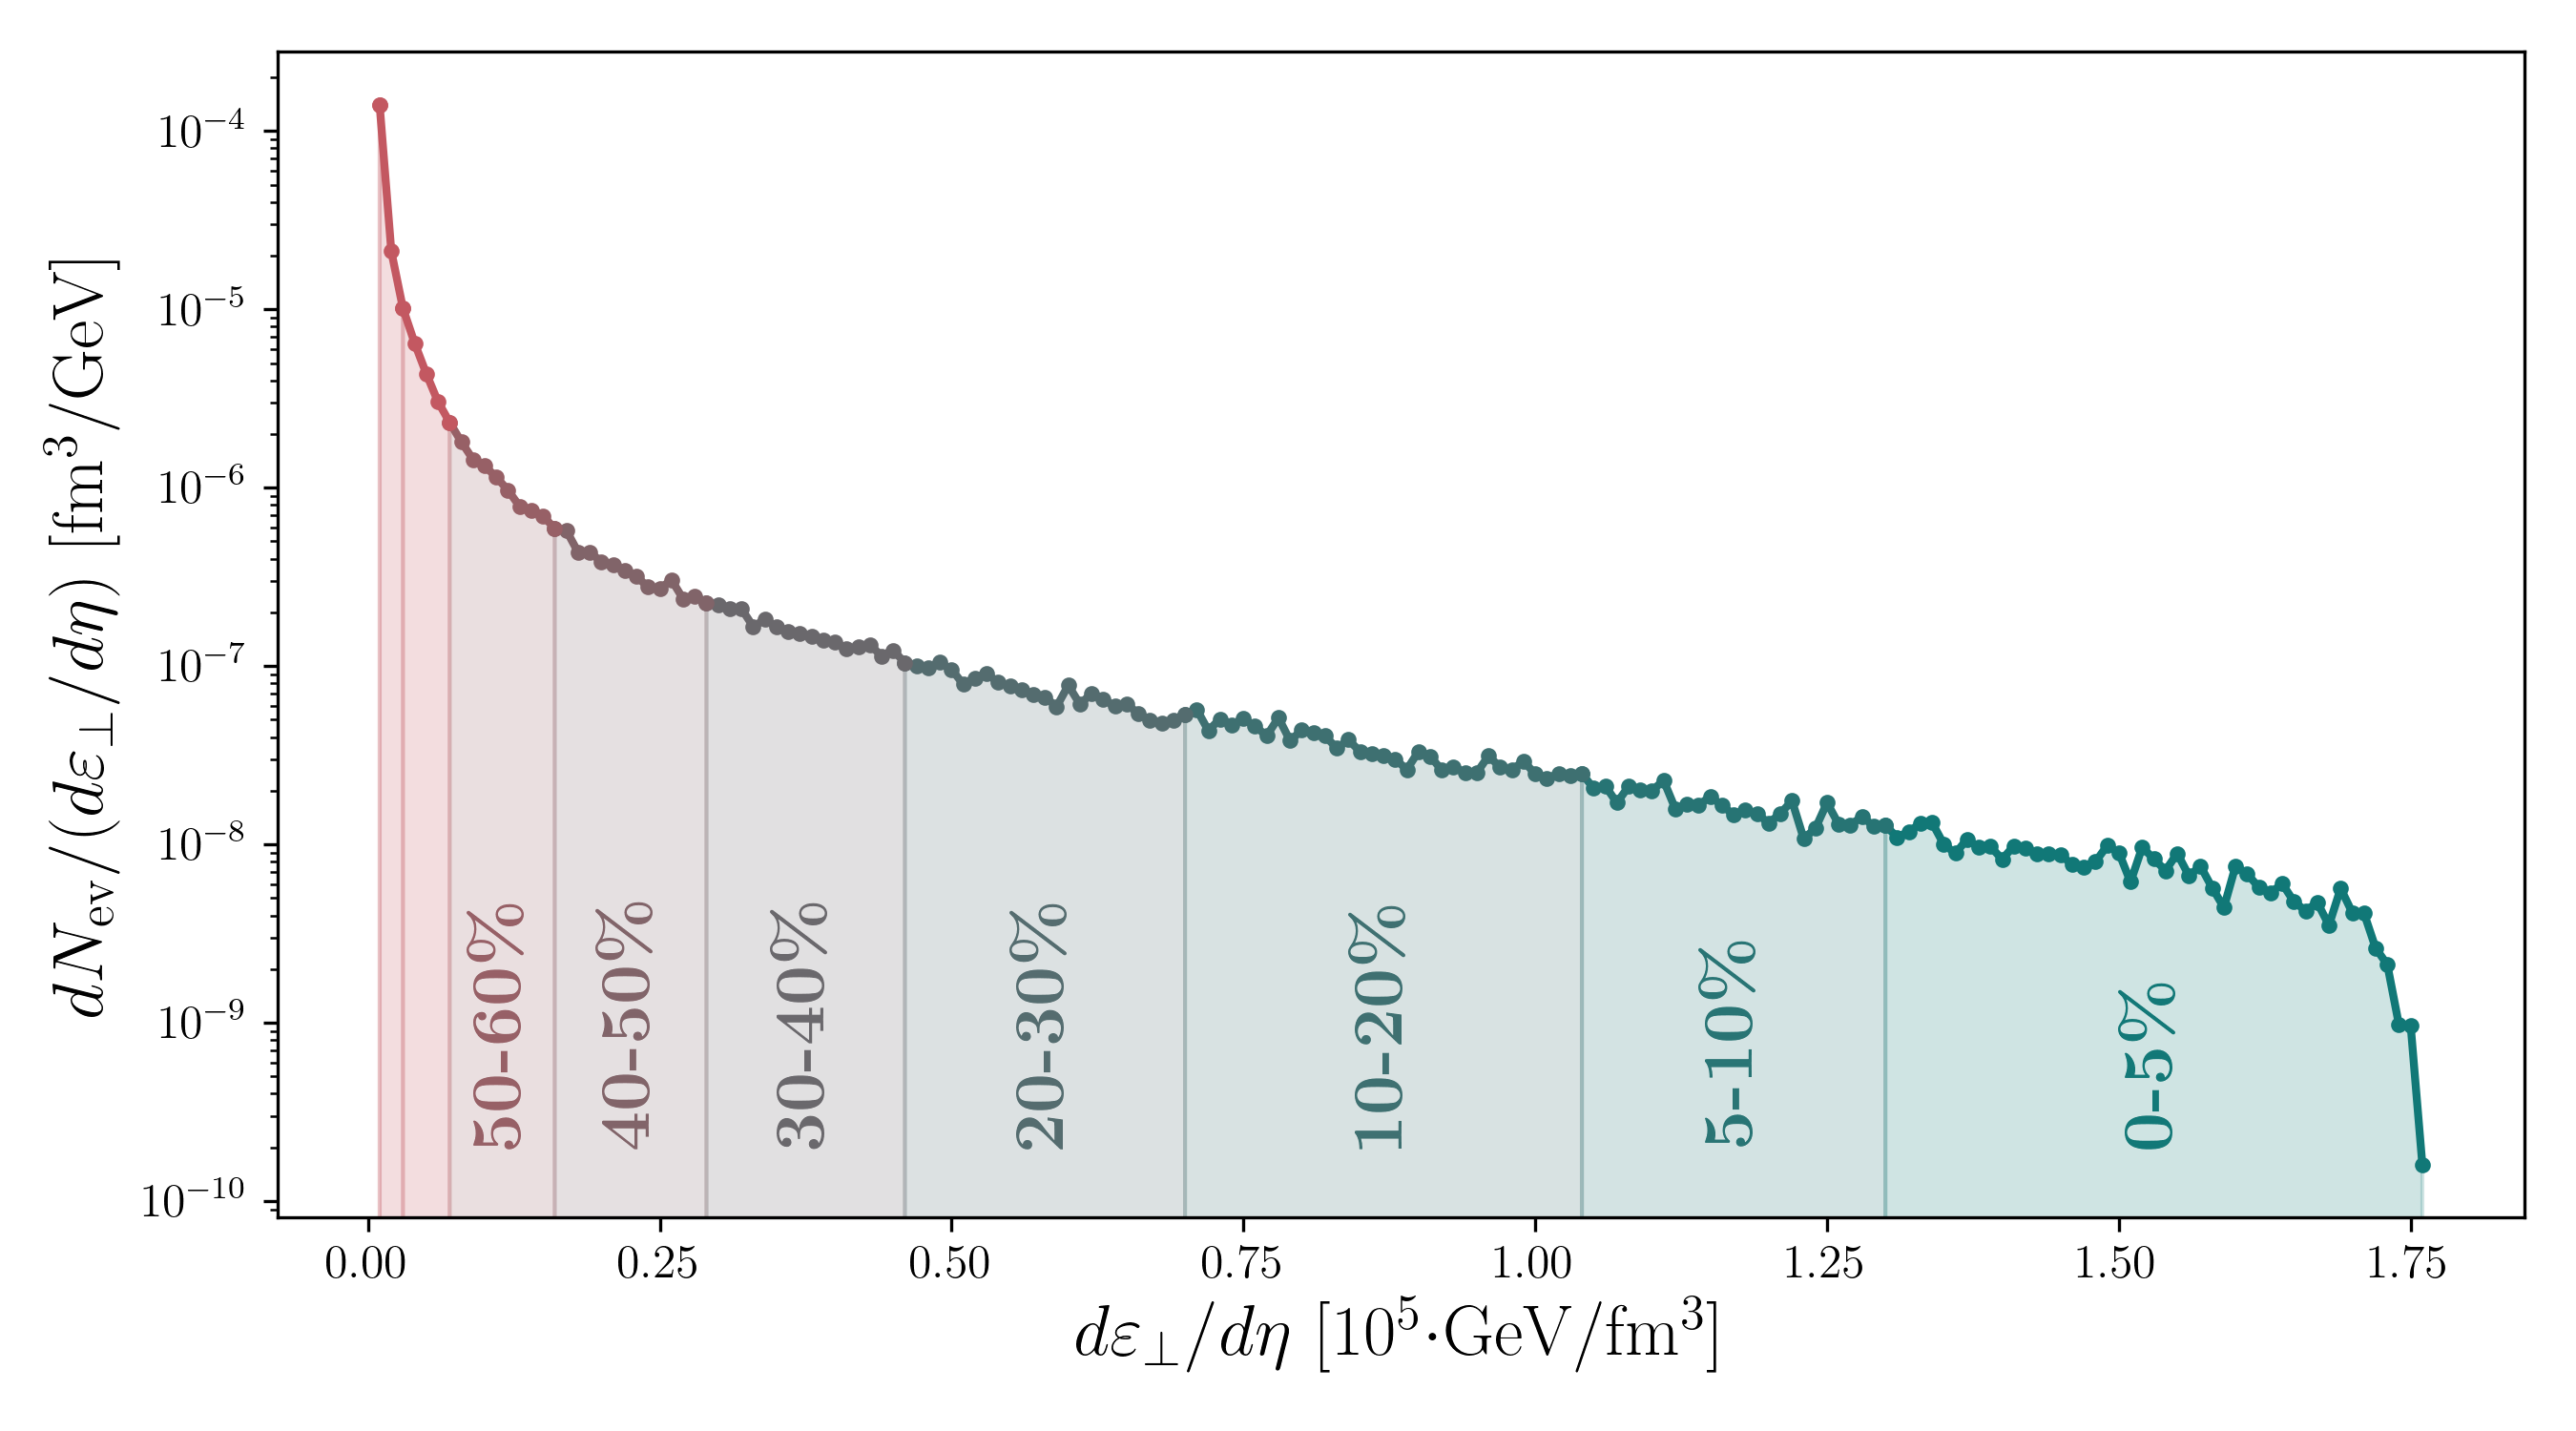
\includegraphics{images/centrality_cut.png}
	\caption{\normalsize Minimum bias centrality selection using $5\cdot 10^4$ events simulated with {\sffamily Curraun}, divided in centrality classes according to their total energy density in the transverse plane $d\varepsilon_\perp/d\eta$.}
\end{figure*}

Therefore, we shall split the events resulting from {\sffamily Curraun} in terms of the total energy density\sidenote{It's not possible to directly evaluate the overlapping area in the transverse plane $\textsf{S}_\perp$ but one may numerically extract
\begin{align*}
    \frac{1}{\tau}\frac{dE_\perp}{d\eta}\Bigg|_{\tau}=(a_T)^2\frac{d\varepsilon_\perp}{d\eta}\Bigg|_{\tau},
\end{align*}
evaluated at $\tau=0.4$ fm/c, where $d\varepsilon_\perp/d\eta$ is the total energy density in the transverse plane.}$d\varepsilon_\perp/d\eta$. Nevertheless, such an approach turns out to be problematic since, within a model constructed with fields, one may not provide a clear criteria whether a collision event occurs or not. Thus, the $100\%$ centrality cut must be chosen by hand. We shall attempt to guess it though an iterative procedure. Since $d\varepsilon_\perp/d\eta$ is correlated with $dN_\text{ch}/d\eta$, one may vary this cut until the ratios between the total energy density in different centrality cuts match the corresponding experimental multiplicity ratios. A later scaling of the energy density should not affect this centrality selection. It is important to mention that\sidenote{Since the previously mentioned correlation is only approximate.}some events may end up in a different centrality class after the hydrodynamic evolution.

\begin{figure}[!hbt]
	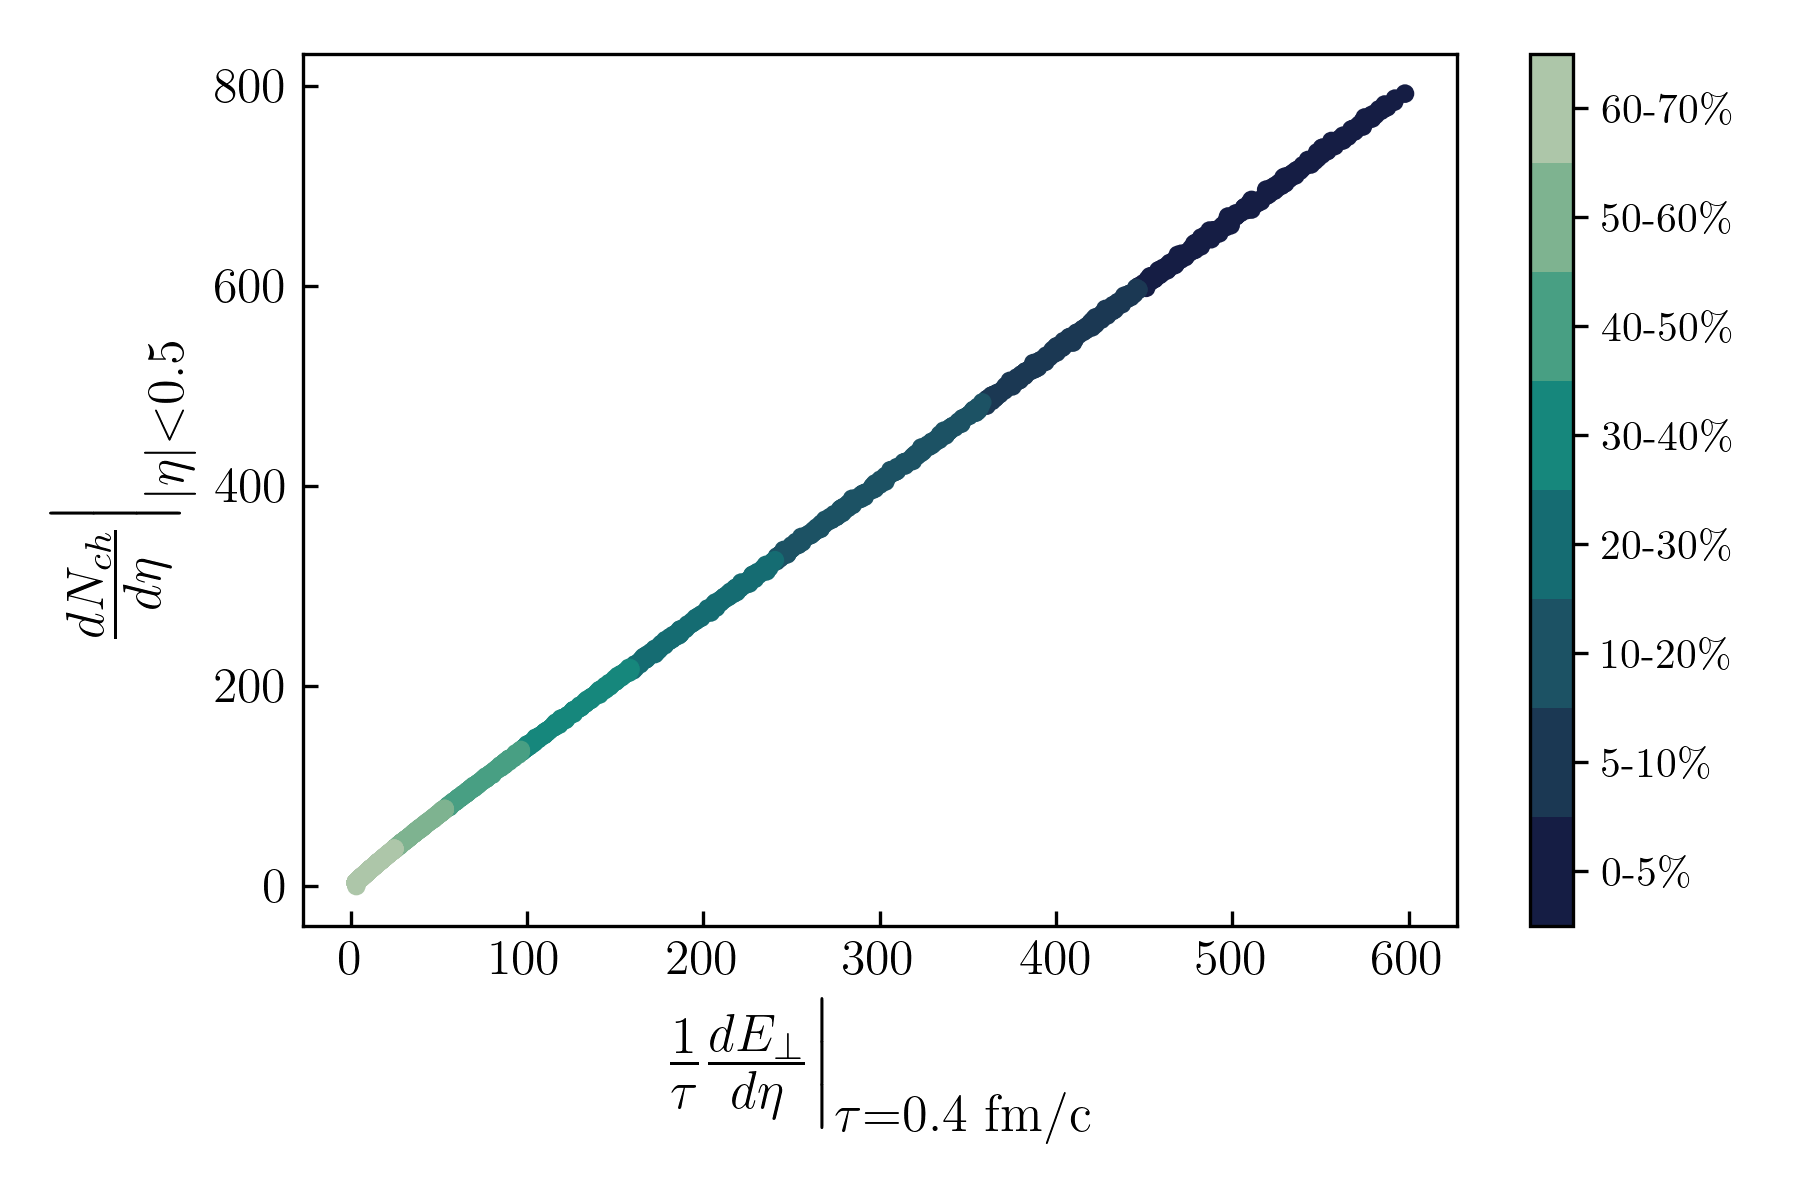
\includegraphics[width=\textwidth]{images/dnch_etot.png}
	\caption{\normalsize Correlation between the initial $d\varepsilon_\perp/d\eta$ and the final $dN_\mathrm{ch}/d\eta$ for a subset of $2700$ events with $300$ events per centrality. Main simulation parameters: $\eta/s=0.24$ and $T_\mathrm{fo}=180$ MeV. A power law fit yields
	\begin{align*}
	    \frac{dN_\text{ch}}{d\eta}\approx 2.1 \left(\frac{1}{\tau}\frac{dE_\perp}{d\eta}\right)^{0.93}.
	\end{align*}
	} 
\end{figure}

\begin{figure}[!hbt]
    \figcolor{tealblue}
	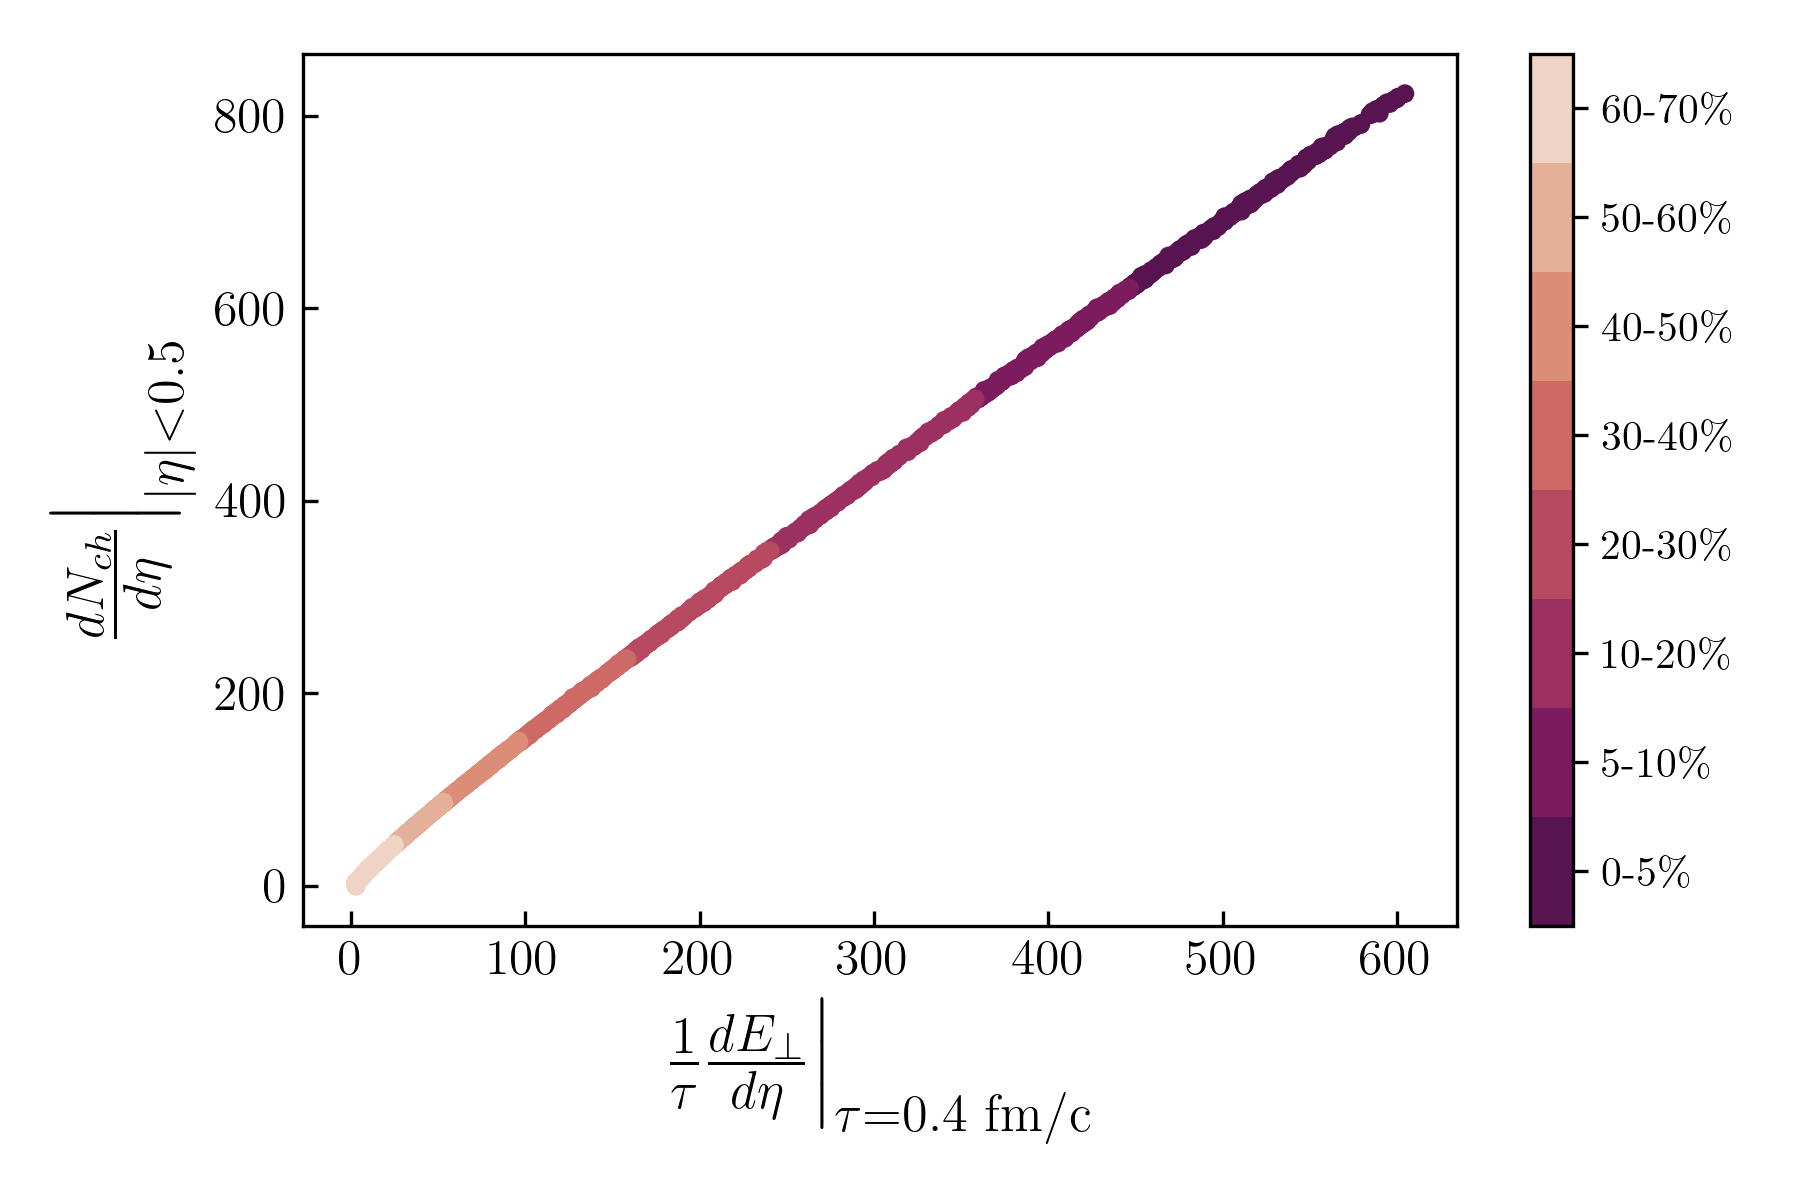
\includegraphics[width=\textwidth]{images/dnch_etot_bulk.png}
	\caption{\normalsize Correlation between the initial $d\varepsilon_\perp/d\eta$ and the final $dN_\mathrm{ch}/d\eta$ for a subset of $2700$ events with $300$ events per centrality. Main simulation parameters: $\eta/s=0.1$ and $T_\mathrm{fo}=180$ MeV and hard-coded $\zeta(T)$. A power law fit yields
	\begin{align*}
	    \frac{dN_\text{ch}}{d\eta}\approx 1.56 \left(\frac{1}{\tau}\frac{dE_\perp}{d\eta}\right)^{0.96}.
	\end{align*}
	} 
\end{figure}

An alternative approach \cite{mcdonaldhydro} would be to take a subset from the total events, pass them trough the hydrodynamic simulation, extract the final multiplicities and then map\sidenote{And obtain a parametrization of the type
\begin{align*}
    \frac{dN_\text{ch}}{d\eta}=\mathrm{const}\left(\frac{1}{\tau}\frac{dE_\perp}{d\eta}\right)^\text{power}.
\end{align*}
}$dN_\text{ch}/d\eta$ as a function of $d\varepsilon_\perp/d\eta$. Afterwards, one may perform a centrality selection using this map. The disadvantage would be that such a map and hence the centrality selection depends on the parameters from the hydrodynamic simulation. 
